
\section{Kwantowe modyfikacje w równaniu Boltzmanna}

\subsection{Zakres stosowalności równania Boltzmanna}
\subsubsection{Równanie Boltzmanna}
Równanie Boltzmanna przedstawia się następującym równaniem:
\begin{equation}
\partial_t f\rpt+\vec{v}\cdot\nab{\r}f\rpt 
+ q\vec{E}\cdot\nab{\p}f\rpt=\underbrace{f\rpt-f_0\rpt}_{\tau(\p)}
\end{equation}
gdzie człon $q\vec{E}\cdot\nab{\p}f\rpt$ to siła Lorentza po zaniedbaniu pola magnetycznego $\B$.\\
Zakładamy, że mamy do czynienia ze zwyrodniałym gazem elektronowym, zatem:
\begin{itemize}
\item ładunek to ładunek elektronu:
\begin{equation} q=-e \end{equation}
\item początkowy rozkład to rozkład Fermiego-Diraca:
\begin{equation} f_0\rpt=f_{FD}(E)=f_{FD}(p)\end{equation}
\item tzw. miara oddziaływania między elektronami, wprowadzona na poprzednim wykładzie:
\begin{equation}
\tau^{-1}(\p)=\sum_{\p'} Q_{pp'}\end{equation}
\end{itemize}
Dzisiejszym celem jest obliczenie $Q_{pp'}$.\\
\subsubsection{Funkcja falowa}
Funkcja falowa w ujęciu kwantowym przedstawia się wzorem:
\begin{equation} \psi_p(\r,t)=\frac{1}{\sqrt{V}}e^{\frac{i}{\hbar}\r\cdot\p-i\omega t}
\end{equation}
Taka funkcja falowa ma wadę - w całej objętości $V=L_xL_yL_z$:
\begin{center}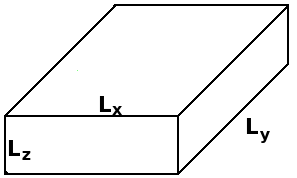
\includegraphics[scale=0.5]{obrazki/wykl_8_obrazek0.png}\end{center}
 gęstość prawdopodobieństwa znalezienia cząstki opisanej funkcją falową $\psi$ jest stała:
\begin{equation}\rho_p(\r,t)=|\psi_p(\r,t)|^2=\psi^*(\r,t)\psi(\r,t)=\frac{1}{V}
\end{equation}
a to oznacza, że prawdopodobieństwo znalezienia elektronu jest wszędzie takie samo- czyli elektron jest zdelokalizowany. 

Nie można się na to zgodzić w przedstawianym toku rozważań, ponieważ jest on prowadzony w podejściu klasycznym.\\
Należy zatem skonstruować nową funkcję falową:
\begin{equation}\chi(\r)=\sum_p C_pe^{\frac{i}{\hbar}\p\cdot\r} \xrightarrow{\p-\text{ciągłe}}\int dp \,C_p\,e^{\frac{i}{\hbar}\p\cdot\r}
\end{equation}
Ostateczne wyrażenie jest transformatą Fouriera, a $C(p)$ to funkcja kształtu. Wybieramy ją w postaci gaussianu (bo gaussian jest prosty):
\begin{equation}C(p)=Ae^{-\frac{(p-p_{_F})^2}{2\Delta p^2}}
\end{equation}
Wtedy:
\begin{equation}\chi(\r)=A\int dp\,e^{-\frac{(p-p_{_F})^2}{2\Delta p^2}}e^{\frac{i}{\hbar}{\p\cdot\r}}
\end{equation}
Wiadomo, że transformata Fouriera z gaussianu to gaussian, czyli $\chi(\r)$ jest pewnym gaussianem, zatem gęstość prawdopodobieństwa nie będzie już stała w całej objętości, czyli elektrony nie będą już zdelokalizowane- teraz będą kulkami o rozmyciu $\Delta r$:\\
\begin{center}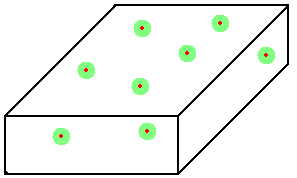
\includegraphics[scale=0.7]{obrazki/wykl_8_obrazek1.png}\end{center}
\subsubsection{Kryterium stosowalności równania Boltzmanna}
Dla "zwykłej" funkcji falowej $\psi$ spełniona jest komutacja: 
\begin{equation}[\hat{H},\hat{p}]=\hat{0}\end{equation}
zatem operatory energii i pędu mają wspólny ciąg funkcji własnych- są to fale płaskie. Ponadto, z własności komutacji, skoro operatory energii i pędu ze sobą komutują, to oznacza, że mogą być określone dokładnie w jednym momencie (nie obowiązuje ich zasada nieoznaczoności Heisenberga).\\
Teraz, w funkcji falowej $\chi$, utraciliśmy tę jednoznaczność. Funkcje płaskie nie są już funkcjami bazowymi operatora pędu $\hat{p}$, zatem  pęd nie jest dobrze określony. Dobrze określone są za to pęd Fermiego i wektor falowy Fermiego :
\begin{equation}p_{_F}=\hbar k_{_F}=\hbar\frac{2\pi}{\lambda_{F}}\end{equation}
\begin{equation}k_{_F}=\sqrt[3]{3\pi n}\end{equation}
gdzie $n$ to gęstość elektronowa.\\
Uwzględniamy też relację nieoznaczoności oraz relację de Broglie'a:
\begin{equation}\Delta p\Delta x \ge \hbar\end{equation}
\begin{equation} \Delta p=\hbar\Delta k\end{equation}
Stąd:
\begin{equation}\Delta x \Delta k \ge 1\end{equation}
gdzie $\Delta x$ to rozmycie pakietu falowego $\Delta r$ w przypadku 1-wymiarowym.\\
Pamiętajmy, że zakładamy, że mamy do czynienia z gazem Lorentza, w którym, w odróżnieniu od gazu idealnego, elektrony rozpraszają się na centrach rozpraszania:
\begin{center}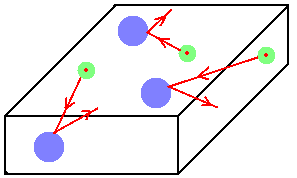
\includegraphics[scale=0.7]{obrazki/wykl_8_obrazek2.png}\end{center}
Elektrony między zderzeniami pokonują średnią drogę swobodną:
\begin{equation}l \propto n^{-\frac{1}{3}}_{imp} \end{equation}
gdzie $n_{imp}$ to gęstość centrów rozpraszania ($imp$- bo traktujemy to jako zaburzenie).\\
Droga swobodna musi być oczywiście dużo większa od "rozmiaru" elektronu, czyli jego parametru rozmycia $\Delta x$:
\begin{equation}\frac{l}{\Delta x}\gg 1\end{equation}
zatem:
\begin{equation}l\Delta k \gg 1\end{equation}
więc również:
\begin{equation}l\Delta k_{_F} \gg 1\end{equation}
Jest to tzw.\textbf{ kryterium Joffego-Regla}, które określa kiedy można stosować równanie Boltzmanna.\\
Dalsze przekształcenia:
\begin{equation}\frac{2\pi}{\lambda_{_F}}l\gg 1~~~ \Rightarrow~~~ \frac{l}{\lambda_{_F}}\gg 1\end{equation}
Ostatecznie:
\begin{equation}l \gg \lambda_{_F}\end{equation}
czyli droga swobodna jest dużo większa od długości fali de Broglie'a elektronu. Wynika stąd, że stosując równanie Boltzmanna, wycinamy efekty kwantowe wynikające z interferencji fal kwantowych. Inaczej: elektron żyje od zderzenia do zderzenia i nie pamięta, co było wcześniej. To tzw. \textbf{proces Markowa}. "Taki prosty obraz jest ukryty w równaniu Boltzmanna".
\subsubsection{Zakresy stosowalności transportu elektronowego}
\begin{itemize}
\item[1.] transport dyfuzyjny (niekoherentny)
\begin{equation}\lambda_{_F} \ll L_\phi < l < L\end{equation}
gdzie kolejno:
	\begin{itemize}
	\item $\lambda_{_F}$ - długość fali Fermiego
	\item $L_\phi$ - długość koherencji (długość, na której elektron wie coś o swojej przeszłości - elektron wie, w jaki sposób uległ rozproszeniu, póki znów się nie rozproszy)
	\item $l$- średnia droga swobodna
	\item $L$ - rozmiar liniowy układu
	\end{itemize}
\item[2.] transport koherentny- "transport z pamięcią":
\begin{equation}\lambda_{_F} \ll l < L_\phi <L\end{equation}
\item[3.] transport balistyczny (formuły Landauera)- elektron nie spotyka centrów rozpraszania:
\begin{equation}\lambda_{_F} \ll L < <l< L_\phi \end{equation}
\item[4.] transport kwazibalistyczny \\
Analogicznie jak transport balistyczny, z tym że dopuszcza się odbicia elektronu od ścianek.
\end{itemize}
\begin{center}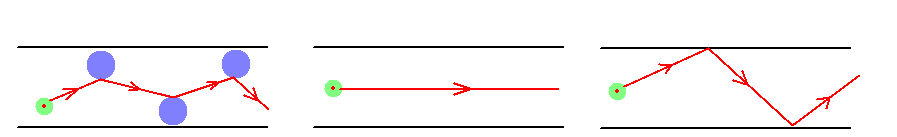
\includegraphics[scale=0.5]{obrazki/wykl_8_obrazek3.png}\\
\textit{transport koherentny ~~~~~transport balistyczny~~~~ transport kwazibalistyczny}
\end{center}
\subsection{Elementy teorii przejść kwantowych- obliczenie elementu $Q_{pp'}$}
\subsubsection{Ustalenie hamiltonianu i równania Schroedingera}
Załóżmy, że układ jest scharakteryzowany przez hamiltonian układu niezaburzonego $\hat{H}_0$ - czyli punktem wyjścia jest transport balistyczny (w 3D).\\
Równanie własne (czyli bezczasowe równanie Schroedingera):
\begin{equation} \hat{H}_0\phi_n(\r)=E_n\phi_n(\r)\label{w8h0}\end{equation}
przy czym $\hat{H}_0$ niekoniecznie jest hamiltonianem swobodnego elektronu- może być w jakimś potencjale, ale nie może się z niczym zderzać.\\
Nakładamy warunek normalizacji:
\begin{equation}\int d^3r\phi_m^*(\r)\phi_n(\r)=\delta_{mn}\end{equation}
i warunek zupełności.\\
Ewolucja czasowa funkcji falowej (czyli rozwiązanie czasowego równania Schroedingera):
\begin{equation}\phi(\r,t)=\phi_n(\r)e^{-\frac{i}{\hbar}E_nt}\end{equation}
Gęstość prawdopodobieństwa:
\begin{equation}\rho_n(\r,t)=|\phi_n(\r)|^2\end{equation}
gdzie:
\begin{equation}|\phi_n(\r)|=\sqrt{\rho_n(\r,t)}\end{equation}
Poddajemy układ $\hat{H}_0$ zaburzeniu $\lambda\hat{V}(t)$:
\begin{equation}\hat{H}_0+\lambda\hat{V}(t)\equiv \hat{H}\end{equation}
gdzie $\hat{V}$ to "potencjał" zaburzający, a $\lambda$ to "parametr małości".\\
Równanie Schroedingera zależne od czasu dla powyższego hamiltonianu:
\begin{equation}i\hbar\partial_t\psi(\r,t)=\hat{H}(t)\psi(\r,t)\end{equation}
Postulujemy:
\begin{equation}\psi(\r,t)=\sum_n C_n(t)e^{-\frac{i}{\hbar}E_nt}\phi_n(\r)\end{equation}
Wprowadzamy oznaczenie:
\begin{equation}\omega_n\equiv \frac{E_n}{\hbar}\end{equation}
Ostatecznie więc w równaniu Schroedingera:
\begin{equation}i\hbar\frac{\partial}{\partial t} \big[
\sum_n C_n e^{-i\omega_n t}\phi_n(\r) \big]=
\big[\hat{H}_0+\lambda\hat{V}(t)\big] 
\sum_n C_n(t)e^{-\omega_n t}\phi_n(\r)\end{equation}
Rozwiążmy to równanie.
\subsubsection{Rozwiązanie równania Schroedingera- etap I}
Biorąc pod uwagę równanie (\ref{w8h0}) i wykonując pochodną czasową, z powyższego równania dostajemy:
\begin{equation}i\hbar\sum_n\Big[ \dot{C}_n e^{-i\omega_nt}\phi_n(\r)
-\underline{i\omega_nC_ne^{-i\omega_nt}} \Big]=
\big[\underline{E_n}+\lambda\hat{V}(t)\big]\phi(\r)C_n(t)e^{-i\omega_nt}
\end{equation}
gdzie $\dot{C}$ to pochodna po czasie. Ponieważ $E_n=\omega_n\hbar$, to podkreślone czynniki w powyższym równaniu znoszą się.\\
Tak powstałe równanie scałkujmy obustronnie:
\begin{equation}\sum_n i\hbar \dot{C}_n(t)e^{-i\omega_nt}\phi_n(\r)=\lambda\sum_n \hat{V}(t)\phi_n(\r)C_n(t)e^{-i\omega_nt}~~~~~~~~~~~\Big/\cdot\int d^3r\phi_m^*\nonumber\end{equation}
\begin{equation}\sum_n i\hbar\dot{C}_n(t)e^{-i\omega_nt}\int d^3r \phi_n(\r)\phi_m^*(\r)=
\lambda\sum_n\underbrace{\int d^3r\phi_m^* \hat{V}(t)\phi_n(\r)}_{\text{element macierzowy~} V_{mn}(t)}C_n(t)e^{-i\omega_nt}
\end{equation}
\begin{equation}\sum_n i\hbar\dot{C}_n(t)e^{-i\omega_nt}\delta_{mn}=
\lambda\sum_n V_{mn}(t)C_n(t)e^{-i\omega_nt}
\end{equation}
Z własności delty Kroneckera:
\begin{equation} i\hbar\dot{C}_m(t)e^{-i\omega_mt}=
\lambda\sum_n V_{mn}(t)C_n(t)e^{-i\omega_nt}~~~~~~~~~~~~~\Big/\cdot e^{i\omega_mt}
\nonumber\end{equation}
\begin{equation} i\hbar\dot{C}_m(t)=
\lambda\sum_n V_{mn}(t)C_n(t)e^{i(\omega_m-\omega_n)t}
\end{equation}
Wprowadźmy oznaczenie:
\begin{equation}\omega_{mn}\equiv \omega_m - \omega_n
\end{equation}
Ostatecznie dostajemy równanie:
\begin{equation} i\hbar\dot{C}_m(t)=
\lambda\sum_n V_{mn}(t)C_n(t)e^{i\omega_{mn}t}
\end{equation}
Powyższy rachunek pozwolił sprowadzić równanie Schroedingera do równania, z którego w kolejnym etapie obliczymy współczynniki $C_n$. Jak później pokażemy, współczynniki te mają kluczową rolę w obliczeniu $Q_{pp'}$.
\subsubsection{Rozwiązanie równania Schroedingera- etap II}
Aby rozwiązać powyższe równanie, załóżmy, że:
\begin{equation} C_m(t)=\sum_{k/0}C_m^{(k)}(t)\lambda^k =
C_m^{(0)}(t) + C_m^{(1)}(t)\lambda +C_m^{(2)}(t)\lambda^2+...
\end{equation}
czyli rozwijamy $C_m$ w szereg. $C^{(k)}$ to $k$-ta pochodna po czasie.\\
Wówczas:
\begin{equation} i\hbar\Big[\dot{C}_m^{(0)}(t)+\lambda\dot{C}_m^{(1)}(t)+\lambda^2\dot{C}_m^{(2)}(t)+...\Big] =
\lambda\sum_nV_{mn}(t)e^{i\omega_{mn}t}\Big[C_m^{(0)}(t) + C_m^{(1)}(t)\lambda +C_m^{(2)}(t)\lambda^2+...\Big]
\end{equation}
Następnie porównujemy elementy z tą samą potęgą $\lambda$-y. Stąd:
\begin{equation}\dot{C}_m^{(0)}(t)=0\end{equation}
\begin{equation}i\hbar\dot{C}_m^{(1)}(t)=\sum_nV_{mn}(t)e^{i\omega_{mn}t}C_m^{(0)}(t)
\label{w8r2}\end{equation}
itd.\\
Załóżmy, że w chwili $t=0$ układ jest w stanie $|k\rangle$, czyli:
\begin{equation}C_m^{(0)}(t=0)=\delta_{mk}\end{equation}
Równanie (\ref{w8r2}):
\begin{equation}\dot{C}_m^{(1)}(t)=\frac{1}{i\hbar}\sum_nV_{mn}(t)e^{i\omega_{mn}t}C_m^{(0)}(t)
\end{equation}
ma następujące rozwiązanie:
\begin{equation}{C}_m^{(1)}(t)-{C}_m^{(0)}(0)=\frac{1}{i\hbar}\int_0^t dt'\sum_nV_{mn}(t')e^{i\omega_{mn}t'}C_m^{(0)}(t')
\end{equation}
\begin{equation}{C}_m^{(1)}(t)=\delta_{mk}+\frac{1}{i\hbar}\int_0^t dt'\sum_nV_{mn}(t')e^{i\omega_{mn}t'}C_m^{(0)}(t')
\end{equation}
Gdy przechodzimy ze stanu $m$ do stanu $k$, to $\delta_{mk}=0$ dla $m\neq k$. Zatem:
\begin{equation}{C}_m^{(1)}(t)=\frac{1}{i\hbar}\int_0^t dt'\sum_nV_{mn}(t')e^{i\omega_{mn}t'}C_m^{(0)}(t')
\end{equation}
Powyższe równanie to równanie całkowe, które rozwiążemy metodą całkową:
\begin{equation}{C}_m^{(1)}(t)=\frac{1}{i\hbar}\int_0^t dt'\sum_nV_{mn}(t')e^{i\omega_{mn}t'}\delta_{nk}
\end{equation}
\begin{equation}{C}_m^{(1)}(t)=\frac{1}{i\hbar}\int_0^t dt'V_{mk}(t')e^{i\omega_{mk}t'}
\end{equation}
Niech element macierzowy przejścia ze stanu $m$ do $k$ będzie stały w czasie:
\begin{equation} V_{mk}(t)=V_{mk}\end{equation}
Wówczas:
\begin{equation}{C}_m^{(1)}(t)=\frac{1}{i\hbar}\int_0^t dt'V_{mk}(t')e^{i\omega_{mk}t'}=\frac{2\pi}{i\hbar}V_{mk}\cdot \frac{1}{2\pi}\underbrace{\int_0^t dt' e^{i\omega_{mk}t'}}_{\delta(\omega_{mk})}
\end{equation}
gdzie ${\delta(\omega_{mk})}$ to delta Diraca. Zatem:
\begin{equation}
C_m^{(1)}(t)=\frac{1}{i\hbar}\int_0^t dt'V_{mk}(t')e^{i\omega_{mk}t'}=\frac{2\pi}{i\hbar}V_{mk}\delta(\omega_{mk})
\end{equation}
Pamiętamy, że współczynniki $C_m$ to współczynniki rozwinięcia funkcji falowej $\psi(\r)$:
\begin{equation}\psi(\r)=\sum_k C_k\phi_k(\r) \label{w8r3}
\end{equation}
Zatem znajdując współczynniki $C_m$, znaleźliśmy rozwiązanie równania Schroedingera w postaci formuły (\ref{w8r3}) na funkcję falową.
\subsubsection{Znaczenie współczynników $C_m$}
Całkując obustronnie równanie (\ref{w8r3}):
\begin{equation}\psi(\r)=\sum_k C_k\phi_k(\r) ~~~~~~~~~~~~~~~\Big/\int d^3r\phi_m^*(\r)\nonumber
\end{equation}
\begin{equation}\int d^3r\phi_m^*(\r)\psi(\r)=\sum_k C_k\int d^3r\phi_m^*(\r)\phi_k(\r)
\end{equation}
\begin{equation}\int d^3r\phi_m^*(\r)\psi(\r)=\sum_k C_k\delta_{mk}
\end{equation}
\begin{equation}\int d^3r\phi_m^*(\r)\psi(\r)=C_m\end{equation}
Zatem $C_m$ to amplituda prawdopodobieństwa wystąpienia stanu $\phi_m$ w superpozycji stanów własnych $\phi$, czyli $\psi$. Natomiast
\begin{equation}|C_m|^2\equiv P_m\end{equation}
to prawdopodobieństwo wystąpienia tego stanu.\\
W ten sposób:
\begin{equation}|C_m^{(1)}(t)|^2\equiv P_m(t)\end{equation}
to prawdopodobieństwo przejścia ze stanu $k$ do stamu $m$.\\
Zatem:
\begin{equation}P_m(t)=|\frac{2\pi}{i\hbar}V_{mk}\delta(\omega_{mk})|^2|=
\frac{4\pi^2}{\hbar^2}|V_{mk}|^2\delta^2(\omega_{mk})=...
\end{equation}
Następnie wykonuje się szereg przekszłtaceń (których nie przedstawiono na wykładzie), m.in zastąpienie: $\delta\rightarrow \frac{sin(kx)}{kx}$, scałkowanie i inne przekształcenia. Uzyskuje się:
\begin{equation}
P_m(t)=\frac{4\pi^2}{\hbar^2}|V_{mk}|^2\frac{\delta(\omega_{mk})}{2\pi}\lim_{T\rightarrow \infty} T
\end{equation}
\subsubsection{Obliczenie współczynników $Q_{pp'}$}
Prawdopodobieństwo przejścia ze stanu $k$ do stanu $m$ na jednostkę czasu to:
\begin{equation}\Gamma_{k\rightarrow m}=\lim_{T\rightarrow\infty}\frac{P_m(t)}{T}=
\frac{4\pi^2}{\hbar^2}|V_{mk}|^2\frac{\delta(\omega_{mk})}{2\pi}
\end{equation}
\begin{equation}\Gamma_{k\rightarrow m}=
\frac{2\pi}{\hbar^2}|V_{mk}|^2{\delta(\omega_{mk})}
\end{equation}
Pamiętamy, że $\omega_{mk}\equiv \omega_m - \omega_k=\frac{E_m-E_k}{\hbar}$, zatem:
\begin{equation}\Gamma_{k\rightarrow m}=
\frac{2\pi}{\hbar^2}|V_{mk}|^2{\delta\Big(\frac{E_m-E_k}{\hbar}\Big)}
\end{equation}
Z właśności delty Diraca:
\begin{equation}\Gamma_{k\rightarrow m}=
\frac{2\pi}{\hbar}|V_{mk}|^2{\delta\Big(E_m-E_k\Big)}
\end{equation}
W końcu miara oddziaływania między elektronami, wprowadzona na poprzednim wykładzie:
\begin{equation}\frac{1}{\tau}\equiv\sum_{p'}Q_{p'p}\end{equation}
to:
\begin{equation}\frac{1}{\tau}=\frac{1}{\Omega}\sum_{p'}\Gamma_{p\rightarrow p'}=
\frac{1}{\Omega}\sum_{p'}\frac{2\pi}{\hbar}|V_{mk}|^2{\delta\Big(E_m-E_k\Big)}
\end{equation}
"Uciąglamy" $p'$:
\begin{equation}\frac{1}{\tau}=
\frac{1}{\Omega}\frac{\Omega}{(2\pi)^3}\int d^3p'\frac{2\pi}{\hbar}|V_{mk}|^2{\delta\Big(E_m-E_k\Big)}
\end{equation}
\begin{equation}\frac{1}{\tau}=
\frac{1}{(2\pi)^2\hbar}\int d^3p'|V_{mk}|^2{\delta\Big(E_m-E_k\Big)}
\end{equation}
Jeżeli założymy, że $\phi_m$ to fale płaskie, to:
\begin{equation}E_p=\frac{p^2}{2m}\end{equation}
Zatem:
\begin{equation}\frac{1}{\tau}=
\frac{1}{(2\pi)^2\hbar}\int d^3p'|V_{mk}|^2{\delta\Big(\frac{p^2-(p')^2}{2m}\Big)}
\end{equation}
W tym miejscu dr Spisak zaleca przeanalizować zadanie z książki "Wybrane rozdziały MMF- rozwiązane problemy", w którym zakłada się potencjał w kształcie delty Diraca. Niestety nie znalazłam tego zadania.
